\documentclass{article}[12pt, a4paper]
\topmargin = 15pt

\usepackage{graphics}
\usepackage[top=1.25in, bottom=1.25in, left=44mm, right=44mm]{geometry}
\usepackage[hidelinks]{hyperref}
\usepackage[utf8]{inputenc}
\usepackage{parskip}

%\VignetteIndexEntry{Upgraining atlas data guide}
%\vignetteDepends{downscale}

\graphicspath{{figures/}}






\usepackage{Sweave}
\begin{document}
\Sconcordance{concordance:Upgraining.tex:Upgraining.Rnw:%
1 19 1 1 6 180 1}


\title{Upgraining atlas data for downscaling: \\ threshold selection using \texttt{upgrain.threshold}}
\author{Charles J. Marsh}
\date{\today}
\maketitle

In order to \texttt{downscale} we need to \texttt{upgrain} our atlas data across several scales (grain sizes). These are then the data points used to fit our \texttt{downscale} models, which can then be extrapolated to predict occupancy at finer grain sizes using \texttt{predict.downscale}. However, if the atlas data is not rectangular, as we aggregate cells during upgraining then the extent also increases (Fig. \ref{fig:Original upgrain}). As the downscaling functions model the change in proportion of occupancy this is undesirable. This document provides a guide to the function \texttt{upgrain.threshold} which aims to advise users on the best way to upgrain atlas data.

\begin{figure}[bth]
\centering
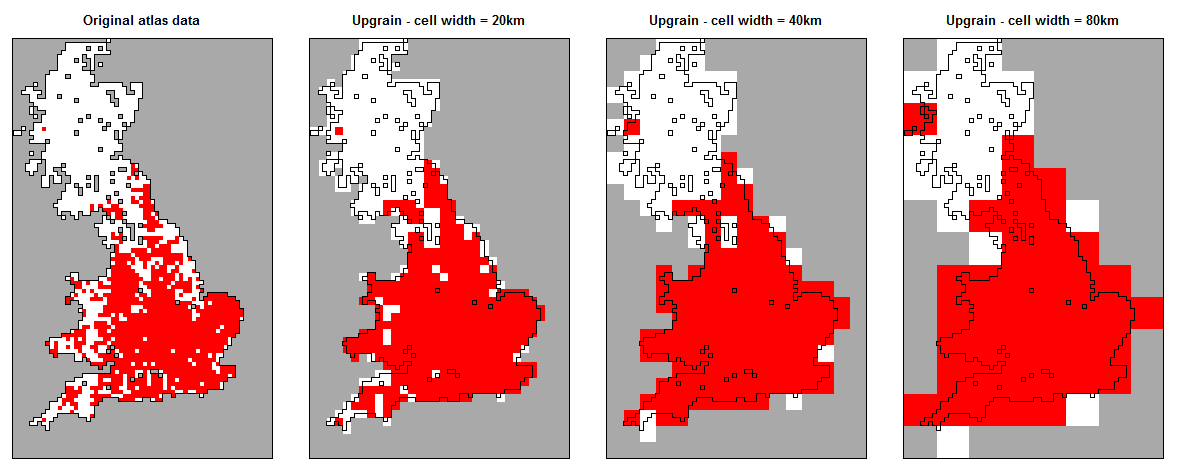
\includegraphics[width=\linewidth]{Original_upgrain.png}
\caption{Upgrained presence (red cells) and absence (white cells) maps for a UK species without standardising extent to the largest grain size. Unsampled cells are dark grey. As we upgrain the atlas data to larger grain sizes the total extent also increases.}
\label{fig:Original upgrain}
\end{figure}

Instead we must ensure the extent is constant across all scales by fixing the extent at all grain sizes to the extent of the largest grain size (Fig. \ref{fig:All interior}). For example, to extend the atlas data we assign unsampled cells that fall within the extent of the largest grain as absences. It is then critically important that after downscaling we \textit{convert our proportion of occupied cells back to area of occupancy by using the standardised extent, not the original atlas data extent}.

\begin{figure}[thb]
\centering
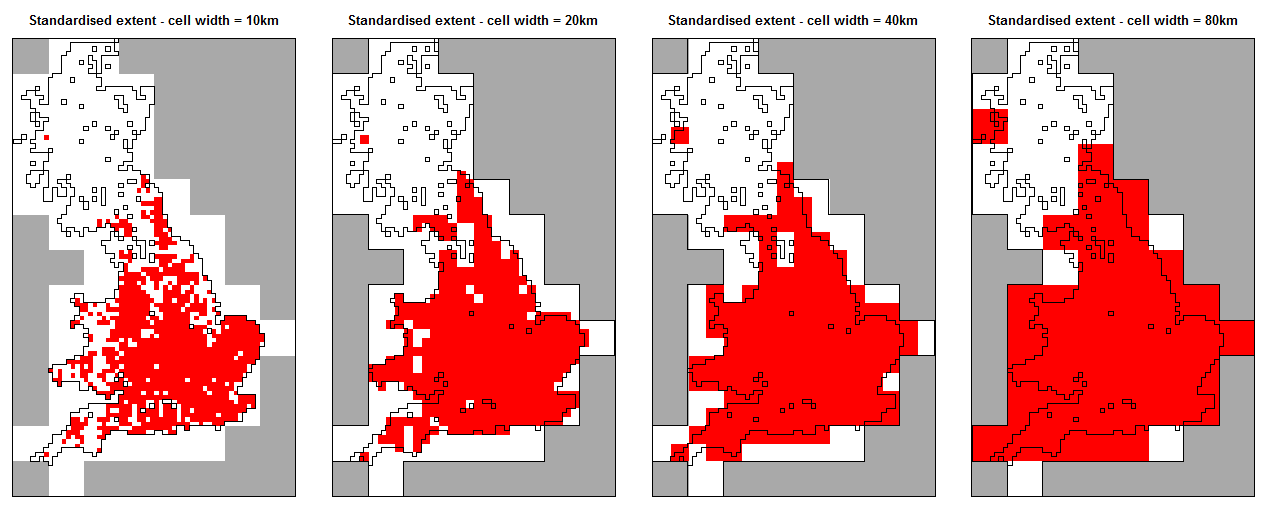
\includegraphics[width=\linewidth]{All_interior.png}
\caption{Upgrained presence (red cells) and absence (white cells) maps for a UK species after standardising extent to the largest grain size. Unsampled cells are dark grey. The extent of the atlas data is extended to that of the largest grain size by assigning absences to unsampled cells.}
\label{fig:All interior}
\end{figure}

However, as we can see in we in figure \ref{fig:All interior}, at the atlas scale we have necessarily assigned unsampled cells as absences (white cells). In the case of the UK the non-surveyed areas are sea and so are probably indeed absences, but in land-locked regions these areas could be suitable habitat for the species.

Instead we may choose to only keep those cells at the largest grain size that fall completely within the surveyed atlas data (Fig. \ref{fig:Interior only}). Therefore no assumptions are made that unsampled cells outside the original atlas data are absences.

\begin{figure}[hbt]
\centering
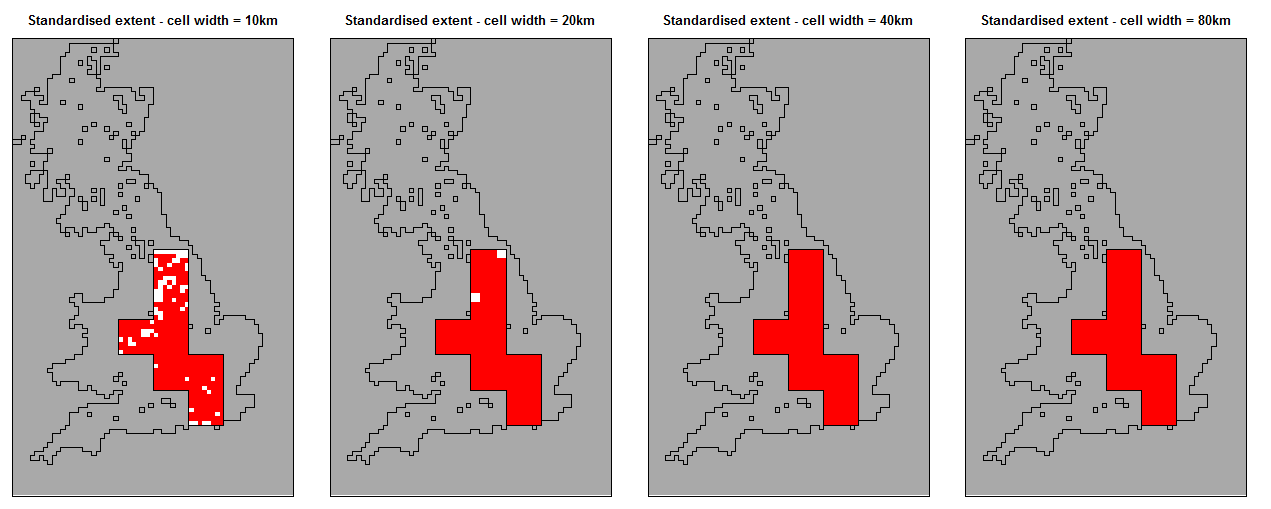
\includegraphics[width=\linewidth]{Interior_only.png}
\caption{Upgrained presence (red cells) and absence (white cells) maps for a UK species after standardising extent to those cells at the largest grain size that solely contain sampled atlas data. Sampled cells outside the selected cells are assigned as No Data (dark grey).}
\label{fig:Interior only}
\end{figure}

Although we no longer make assumptions about unsampled areas, if the shape of the extent is irregular, or if there are unsampled cells within the atlas data, such as here, then this method may exclude a large proportion of the original atlas data, even known presences. This may be particularly pronounced for species that occupy the edges of the extent, such as coastal species, as very few of these edge cells will be retained using such a procedure.

Therefore there is a clear trade-off between assigning large areas of unsampled areas as absence, and discarding sampled areas and known presences. Instead it may be good to apply some threshold where those cells at the largest grain size that only contain a certain amount of unsampled area are disregarded. The \texttt{upgrain.threshold} function allows visualisations of this trade-off at the atlas scale through four plots against threshold (Fig. \ref{fig:Threshold plots}):

\begin{enumerate} \itemsep1pt \parskip0pt 
\item [a.] The total standardised extent;
\item [b.] The number of unsampled cells added and assigned as absences, and the number of sampled cells excluded and assigned as No Data;
\item [c.] The proportion of the original atlas data retained;
\item [d.] The proportion of known presences excluded.
\end{enumerate}

\begin{Schunk}
\begin{Sinput}
> library("downscale")
> #  The data may be a raster layer of presence (1) and absence (0) data 
> #  or a data frame of cell centre coordinates and presence-absence data 
> #  in which case it must have these column names: "lon", "lat", "presence"
> data.file <- system.file("extdata", "atlas_data.txt", package = "downscale")
> atlas.data <- read.table(data.file, header = TRUE)
> names(atlas.data)
\end{Sinput}
\begin{Soutput}
[1] "lon"      "lat"      "presence"

\end{Soutput}
\begin{Sinput}
> thresh <- upgrain.threshold(atlas.data = atlas.data,
+                             cell.width = 10,
+                             scales = 3,
+                             thresholds = seq(0, 1, 0.01))
\end{Sinput}
\end{Schunk}

\begin{figure}[ht]
\centering
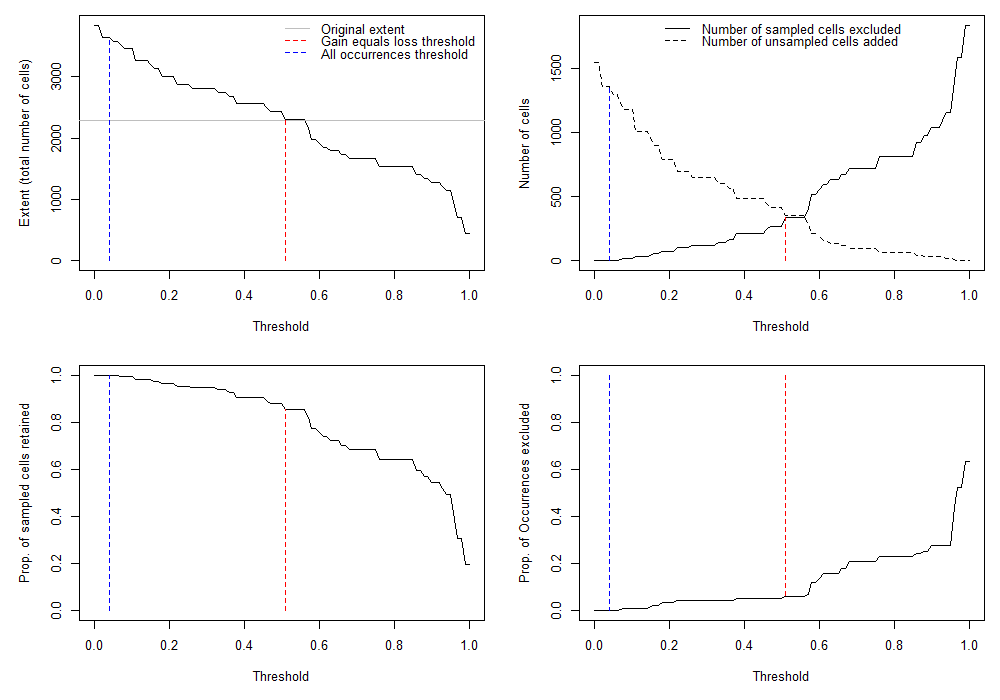
\includegraphics[width=\linewidth]{Threshold_plots.png}
\caption{Diagnostic plots produced by \texttt{upgrain.threshold} used to explore the trade-off  between assigning large areas of unsampled areas as absence, and discarding sampled areas and known presences. Two possible thresholds in the quantity of unsampled area allowed within cells at the largest grain size are identified: the “all\_occurrences” threshold (blue line) and the “gain\_equals\_loss” threshold (red line).}
\label{fig:Threshold plots}
\end{figure}

The user can then take any threshold as the input in the \texttt{upgrain} function, however we have also identified four possibilities for the user: 

\begin{table}[!h]
\centering
\begin{tabular}{ c  c  p{6.2cm} }
\hline \noalign{\smallskip}
Threshold & Name & Description  \\
\hline \noalign{\smallskip}
0 & "All\_Sampled" & All of the original atlas data is included (Fig. \ref{fig:All interior}). \\ [0.2cm]

Blue line & "All\_Occurrences" & The threshold where no occurrences in the atlas data are excluded (Fig. \ref{fig:Threshold plots}d). \\ [0.2cm]

Red line & "Gain\_Equals\_Loss" & The threshold where the number of sampled atlas cells reclassified as No Data equals the number of unsampled exterior cells reclassified as absence (plot b). In this threshold the new standardised extent also equals the extent of the original atlas data (Fig. \ref{fig:Threshold plots}a). \\ [0.2cm]

1 & "Sampled\_Only" & Only cells that contain 100\% sampled atlas data are included (Fig. \ref{fig:Interior only}). \\ [0.1cm]
\hline
\end{tabular}
\end{table}

\begin{Schunk}
\begin{Sinput}
> thresh$Thresholds
\end{Sinput}
\begin{Soutput}
  All_Sampled All_Occurrences Gain_Equals_Loss Sampled_Only
1           0            0.04             0.51            1
\end{Soutput}
\begin{Sinput}
> head(thresh$Data)
\end{Sinput}
\begin{Soutput}
  Threshold SampledExcluded SampledIncluded UnsampledAdded
1      0.00               0            2289           1439
2      0.01               0            2289           1439
3      0.02               3            2286           1306
4      0.03               3            2286           1306
5      0.04               3            2286           1306
6      0.05               6            2283           1301
  Extent PresencesExcluded
1   3840             0.000
2   3840             0.000
3   3648             0.000
4   3648             0.000
5   3648             0.000
6   3584             0.002
\end{Soutput}
\end{Schunk}

Figure \ref{fig:Threshold maps} shows the maps if each of these thresholds were applied. The semi-transparent area within the black polygon are the cells included after applying the threshold. This is overlain on the original atlas data where red = presence, light grey = absence, and dark grey = unsampled cells. The plots allow a visual interpretation of where and how much sampled data is removed and unsampled data added. For example, due to the distribution of our unsampled cells throughout our atlas data, the "Sampled Only" threshold only captures the very central portion of our species distribution.

\begin{figure}[!ht]
\centering
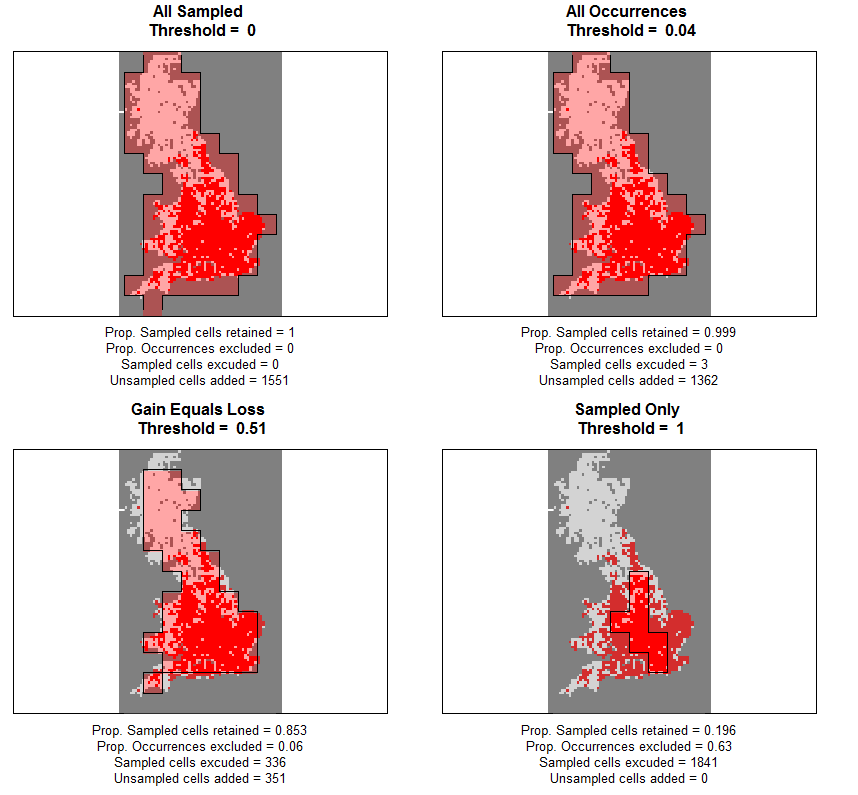
\includegraphics[width=\linewidth]{Threshold_maps.png}
\caption{Maps of the atlas data (red = presence; light grey = absence; unsampled = dark grey) overlain with polygons showing the standardised extent after applying each of four possible thresholds.}
\label{fig:Threshold maps}
\end{figure}

The choice of threshold is therefore dependent upon the shape of the atlas region and the distribution of the species under study. For example, if the atlas region is rectangular then the “Sampled Only” threshold may result in no loss of sampled cells and in fact all four threshold options may be the same. Or if a species is confined to the interior of the region then the “All Occurrences” threshold may equal the “Sampled Only” threshold. Alternatively, for a species confined to the edges of the atlas region then the “All Occurrences” threshold may equal the “All Sampled” threshold. Therefore, we provide no single recommendation, but leave the final choice of threshold to the user to determine on a case-by-case basis.

\end{document}
